\documentclass[1p]{elsarticle_modified}
%\bibliographystyle{elsarticle-num}

%\usepackage[colorlinks]{hyperref}
%\usepackage{abbrmath_seonhwa} %\Abb, \Ascr, \Acal ,\Abf, \Afrak
\usepackage{amsfonts}
\usepackage{amssymb}
\usepackage{amsmath}
\usepackage{amsthm}
\usepackage{scalefnt}
\usepackage{amsbsy}
\usepackage{kotex}
\usepackage{caption}
\usepackage{subfig}
\usepackage{color}
\usepackage{graphicx}
\usepackage{xcolor} %% white, black, red, green, blue, cyan, magenta, yellow
\usepackage{float}
\usepackage{setspace}
\usepackage{hyperref}

\usepackage{tikz}
\usetikzlibrary{arrows}

\usepackage{multirow}
\usepackage{array} % fixed length table
\usepackage{hhline}

%%%%%%%%%%%%%%%%%%%%%
\makeatletter
\renewcommand*\env@matrix[1][\arraystretch]{%
	\edef\arraystretch{#1}%
	\hskip -\arraycolsep
	\let\@ifnextchar\new@ifnextchar
	\array{*\c@MaxMatrixCols c}}
\makeatother %https://tex.stackexchange.com/questions/14071/how-can-i-increase-the-line-spacing-in-a-matrix
%%%%%%%%%%%%%%%

\usepackage[normalem]{ulem}

\newcommand{\msout}[1]{\ifmmode\text{\sout{\ensuremath{#1}}}\else\sout{#1}\fi}
%SOURCE: \msout is \stkout macro in https://tex.stackexchange.com/questions/20609/strikeout-in-math-mode

\newcommand{\cancel}[1]{
	\ifmmode
	{\color{red}\msout{#1}}
	\else
	{\color{red}\sout{#1}}
	\fi
}

\newcommand{\add}[1]{
	{\color{blue}\uwave{#1}}
}

\newcommand{\replace}[2]{
	\ifmmode
	{\color{red}\msout{#1}}{\color{blue}\uwave{#2}}
	\else
	{\color{red}\sout{#1}}{\color{blue}\uwave{#2}}
	\fi
}

\newcommand{\Sol}{\mathcal{S}} %segment
\newcommand{\D}{D} %diagram
\newcommand{\A}{\mathcal{A}} %arc


%%%%%%%%%%%%%%%%%%%%%%%%%%%%%5 test

\def\sl{\operatorname{\textup{SL}}(2,\Cbb)}
\def\psl{\operatorname{\textup{PSL}}(2,\Cbb)}
\def\quan{\mkern 1mu \triangleright \mkern 1mu}

\theoremstyle{definition}
\newtheorem{thm}{Theorem}[section]
\newtheorem{prop}[thm]{Proposition}
\newtheorem{lem}[thm]{Lemma}
\newtheorem{ques}[thm]{Question}
\newtheorem{cor}[thm]{Corollary}
\newtheorem{defn}[thm]{Definition}
\newtheorem{exam}[thm]{Example}
\newtheorem{rmk}[thm]{Remark}
\newtheorem{alg}[thm]{Algorithm}

\newcommand{\I}{\sqrt{-1}}
\begin{document}

%\begin{frontmatter}
%
%\title{Boundary parabolic representations of knots up to 8 crossings}
%
%%% Group authors per affiliation:
%\author{Yunhi Cho} 
%\address{Department of Mathematics, University of Seoul, Seoul, Korea}
%\ead{yhcho@uos.ac.kr}
%
%
%\author{Seonhwa Kim} %\fnref{s_kim}}
%\address{Center for Geometry and Physics, Institute for Basic Science, Pohang, 37673, Korea}
%\ead{ryeona17@ibs.re.kr}
%
%\author{Hyuk Kim}
%\address{Department of Mathematical Sciences, Seoul National University, Seoul 08826, Korea}
%\ead{hyukkim@snu.ac.kr}
%
%\author{Seokbeom Yoon}
%\address{Department of Mathematical Sciences, Seoul National University, Seoul, 08826,  Korea}
%\ead{sbyoon15@snu.ac.kr}
%
%\begin{abstract}
%We find all boundary parabolic representation of knots up to 8 crossings.
%
%\end{abstract}
%\begin{keyword}
%    \MSC[2010] 57M25 
%\end{keyword}
%
%\end{frontmatter}

%\linenumbers
%\tableofcontents
%
\newcommand\colored[1]{\textcolor{white}{\rule[-0.35ex]{0.8em}{1.4ex}}\kern-0.8em\color{red} #1}%
%\newcommand\colored[1]{\textcolor{white}{ #1}\kern-2.17ex	\textcolor{white}{ #1}\kern-1.81ex	\textcolor{white}{ #1}\kern-2.15ex\color{red}#1	}

{\Large $\underline{12a_{0621}~(K12a_{0621})}$}

\setlength{\tabcolsep}{10pt}
\renewcommand{\arraystretch}{1.6}
\vspace{1cm}\begin{tabular}{m{100pt}>{\centering\arraybackslash}m{274pt}}
\multirow{5}{120pt}{
	\centering
	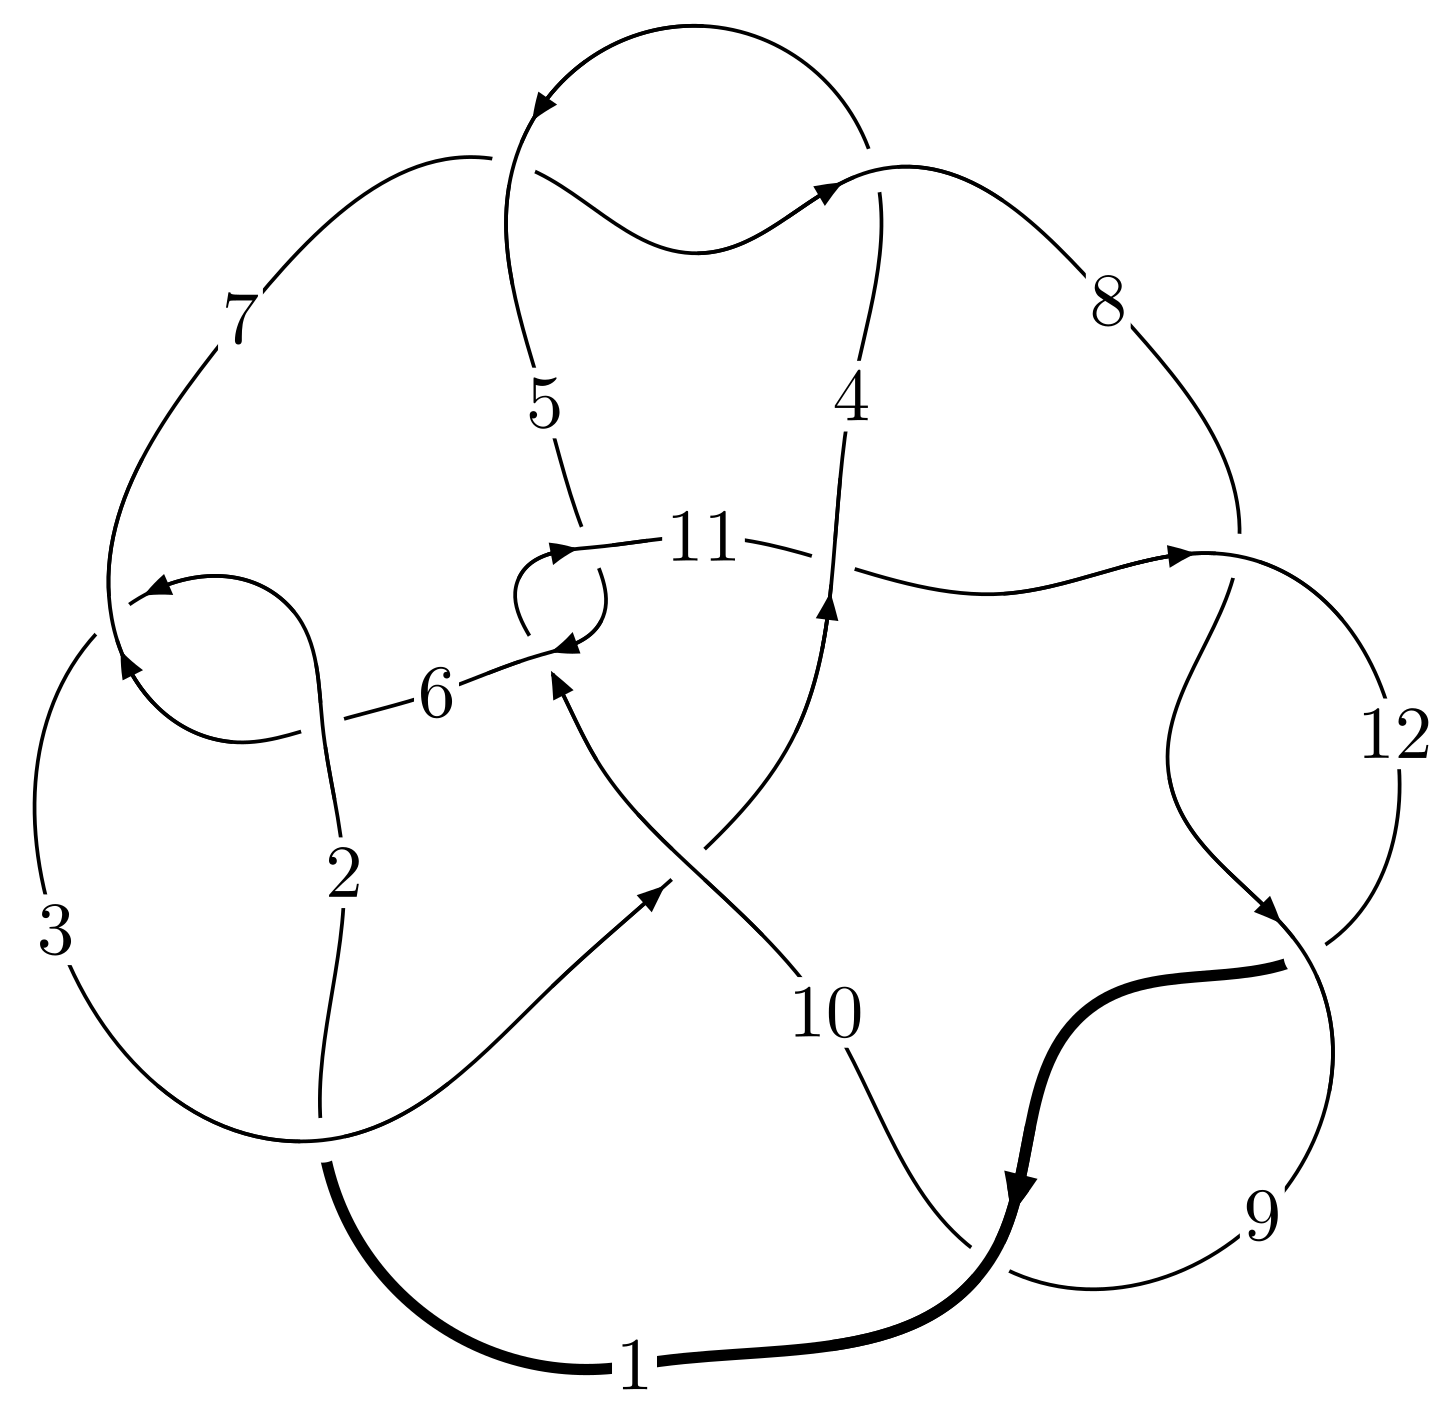
\includegraphics[width=112pt]{../../../GIT/diagram.site/Diagrams/png/1422_12a_0621.png}\\
\ \ \ A knot diagram\footnotemark}&
\allowdisplaybreaks
\textbf{Linearized knot diagam} \\
\cline{2-2}
 &
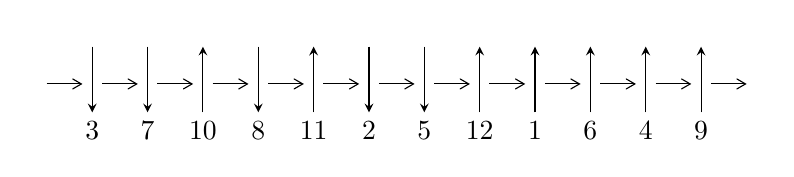
\begin{tikzpicture}[x=20pt, y=17pt]
	% nodes
	\node (C0) at (0, 0) {};
	\node (C1) at (1, 0) {};
	\node (C1U) at (1, +1) {};
	\node (C1D) at (1, -1) {3};

	\node (C2) at (2, 0) {};
	\node (C2U) at (2, +1) {};
	\node (C2D) at (2, -1) {7};

	\node (C3) at (3, 0) {};
	\node (C3U) at (3, +1) {};
	\node (C3D) at (3, -1) {10};

	\node (C4) at (4, 0) {};
	\node (C4U) at (4, +1) {};
	\node (C4D) at (4, -1) {8};

	\node (C5) at (5, 0) {};
	\node (C5U) at (5, +1) {};
	\node (C5D) at (5, -1) {11};

	\node (C6) at (6, 0) {};
	\node (C6U) at (6, +1) {};
	\node (C6D) at (6, -1) {2};

	\node (C7) at (7, 0) {};
	\node (C7U) at (7, +1) {};
	\node (C7D) at (7, -1) {5};

	\node (C8) at (8, 0) {};
	\node (C8U) at (8, +1) {};
	\node (C8D) at (8, -1) {12};

	\node (C9) at (9, 0) {};
	\node (C9U) at (9, +1) {};
	\node (C9D) at (9, -1) {1};

	\node (C10) at (10, 0) {};
	\node (C10U) at (10, +1) {};
	\node (C10D) at (10, -1) {6};

	\node (C11) at (11, 0) {};
	\node (C11U) at (11, +1) {};
	\node (C11D) at (11, -1) {4};

	\node (C12) at (12, 0) {};
	\node (C12U) at (12, +1) {};
	\node (C12D) at (12, -1) {9};
	\node (C13) at (13, 0) {};

	% arrows
	\draw[->,>={angle 60}]
	(C0) edge (C1) (C1) edge (C2) (C2) edge (C3) (C3) edge (C4) (C4) edge (C5) (C5) edge (C6) (C6) edge (C7) (C7) edge (C8) (C8) edge (C9) (C9) edge (C10) (C10) edge (C11) (C11) edge (C12) (C12) edge (C13) ;	\draw[->,>=stealth]
	(C1U) edge (C1D) (C2U) edge (C2D) (C3D) edge (C3U) (C4U) edge (C4D) (C5D) edge (C5U) (C6U) edge (C6D) (C7U) edge (C7D) (C8D) edge (C8U) (C9D) edge (C9U) (C10D) edge (C10U) (C11D) edge (C11U) (C12D) edge (C12U) ;
	\end{tikzpicture} \\
\hhline{~~} \\& 
\textbf{Solving Sequence} \\ \cline{2-2} 
 &
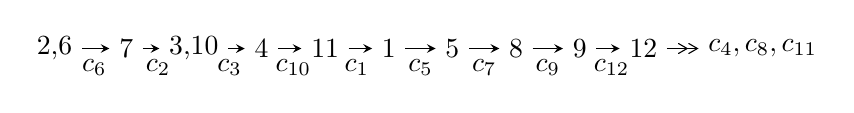
\begin{tikzpicture}[x=23pt, y=7pt]
	% node
	\node (A0) at (-1/8, 0) {2,6};
	\node (A1) at (1, 0) {7};
	\node (A2) at (33/16, 0) {3,10};
	\node (A3) at (25/8, 0) {4};
	\node (A4) at (33/8, 0) {11};
	\node (A5) at (41/8, 0) {1};
	\node (A6) at (49/8, 0) {5};
	\node (A7) at (57/8, 0) {8};
	\node (A8) at (65/8, 0) {9};
	\node (A9) at (73/8, 0) {12};
	\node (C1) at (1/2, -1) {$c_{6}$};
	\node (C2) at (3/2, -1) {$c_{2}$};
	\node (C3) at (21/8, -1) {$c_{3}$};
	\node (C4) at (29/8, -1) {$c_{10}$};
	\node (C5) at (37/8, -1) {$c_{1}$};
	\node (C6) at (45/8, -1) {$c_{5}$};
	\node (C7) at (53/8, -1) {$c_{7}$};
	\node (C8) at (61/8, -1) {$c_{9}$};
	\node (C9) at (69/8, -1) {$c_{12}$};
	\node (A10) at (11, 0) {$c_{4},c_{8},c_{11}$};

	% edge
	\draw[->,>=stealth]	
	(A0) edge (A1) (A1) edge (A2) (A2) edge (A3) (A3) edge (A4) (A4) edge (A5) (A5) edge (A6) (A6) edge (A7) (A7) edge (A8) (A8) edge (A9) ;
	\draw[->>,>={angle 60}]	
	(A9) edge (A10);
\end{tikzpicture} \\ 

\end{tabular} \\

\footnotetext{
The image of knot diagram is generated by the software ``\textbf{Draw programme}" developed by Andrew Bartholomew(\url{http://www.layer8.co.uk/maths/draw/index.htm\#Running-draw}), where we modified some parts for our purpose(\url{https://github.com/CATsTAILs/LinksPainter}).
}\phantom \\ \newline 
\centering \textbf{Ideals for irreducible components\footnotemark of $X_{\text{par}}$} 
 
\begin{align*}
I^u_{1}&=\langle 
-1.20239\times10^{215} u^{107}+1.87947\times10^{215} u^{106}+\cdots+1.06285\times10^{214} b-3.23420\times10^{217},\\
\phantom{I^u_{1}}&\phantom{= \langle  }5.28723\times10^{217} u^{107}-8.28194\times10^{217} u^{106}+\cdots+1.28605\times10^{216} a+1.46385\times10^{220},\\
\phantom{I^u_{1}}&\phantom{= \langle  }u^{108}-2 u^{107}+\cdots+665 u-121\rangle \\
I^u_{2}&=\langle 
u^{20}+2 u^{19}+\cdots+b+5,\;-12 u^{20}-5 u^{19}+\cdots+a-15,\;u^{21}+u^{20}+\cdots+3 u+1\rangle \\
\\
\end{align*}
\raggedright * 2 irreducible components of $\dim_{\mathbb{C}}=0$, with total 129 representations.\\
\footnotetext{All coefficients of polynomials are rational numbers. But the coefficients are sometimes approximated in decimal forms when there is not enough margin.}
\newpage
\renewcommand{\arraystretch}{1}
\centering \section*{I. $I^u_{1}= \langle -1.20\times10^{215} u^{107}+1.88\times10^{215} u^{106}+\cdots+1.06\times10^{214} b-3.23\times10^{217},\;5.29\times10^{217} u^{107}-8.28\times10^{217} u^{106}+\cdots+1.29\times10^{216} a+1.46\times10^{220},\;u^{108}-2 u^{107}+\cdots+665 u-121 \rangle$}
\flushleft \textbf{(i) Arc colorings}\\
\begin{tabular}{m{7pt} m{180pt} m{7pt} m{180pt} }
\flushright $a_{2}=$&$\begin{pmatrix}0\\u\end{pmatrix}$ \\
\flushright $a_{6}=$&$\begin{pmatrix}1\\0\end{pmatrix}$ \\
\flushright $a_{7}=$&$\begin{pmatrix}1\\u^2\end{pmatrix}$ \\
\flushright $a_{3}=$&$\begin{pmatrix}- u\\- u^3+u\end{pmatrix}$ \\
\flushright $a_{10}=$&$\begin{pmatrix}-41.1122 u^{107}+64.3984 u^{106}+\cdots+36653.3 u-11382.6\\11.3129 u^{107}-17.6833 u^{106}+\cdots-9984.50 u+3042.95\end{pmatrix}$ \\
\flushright $a_{4}=$&$\begin{pmatrix}0.827553 u^{107}-2.28938 u^{106}+\cdots-1509.86 u+617.568\\-4.54597 u^{107}+6.83298 u^{106}+\cdots+3815.14 u-1175.67\end{pmatrix}$ \\
\flushright $a_{11}=$&$\begin{pmatrix}-29.7993 u^{107}+46.7151 u^{106}+\cdots+26668.8 u-8339.62\\11.3129 u^{107}-17.6833 u^{106}+\cdots-9984.50 u+3042.95\end{pmatrix}$ \\
\flushright $a_{1}=$&$\begin{pmatrix}u^3\\u^5- u^3+u\end{pmatrix}$ \\
\flushright $a_{5}=$&$\begin{pmatrix}-16.4923 u^{107}+26.9884 u^{106}+\cdots+15115.1 u-4723.79\\22.4428 u^{107}-33.7114 u^{106}+\cdots-18998.4 u+5793.78\end{pmatrix}$ \\
\flushright $a_{8}=$&$\begin{pmatrix}49.2264 u^{107}-75.9538 u^{106}+\cdots-42626.0 u+13138.8\\3.39652 u^{107}-6.09058 u^{106}+\cdots-3073.51 u+962.163\end{pmatrix}$ \\
\flushright $a_{9}=$&$\begin{pmatrix}-42.3987 u^{107}+66.3530 u^{106}+\cdots+37791.9 u-11742.9\\5.22265 u^{107}-8.18612 u^{106}+\cdots-4597.36 u+1378.17\end{pmatrix}$ \\
\flushright $a_{12}=$&$\begin{pmatrix}-20.8291 u^{107}+33.7038 u^{106}+\cdots+19474.8 u-6266.69\\12.6839 u^{107}-20.1507 u^{106}+\cdots-11239.0 u+3449.01\end{pmatrix}$\\&\end{tabular}
\flushleft \textbf{(ii) Obstruction class $= -1$}\\~\\
\flushleft \textbf{(iii) Cusp Shapes $= -44.1834 u^{107}+68.3158 u^{106}+\cdots+39249.5 u-11362.2$}\\~\\
\newpage\renewcommand{\arraystretch}{1}
\flushleft \textbf{(iv) u-Polynomials at the component}\newline \\
\begin{tabular}{m{50pt}|m{274pt}}
Crossings & \hspace{64pt}u-Polynomials at each crossing \\
\hline $$\begin{aligned}c_{1}\end{aligned}$$&$\begin{aligned}
&u^{108}+42 u^{107}+\cdots+640907 u+14641
\end{aligned}$\\
\hline $$\begin{aligned}c_{2},c_{6}\end{aligned}$$&$\begin{aligned}
&u^{108}-2 u^{107}+\cdots+665 u-121
\end{aligned}$\\
\hline $$\begin{aligned}c_{3}\end{aligned}$$&$\begin{aligned}
&u^{108}-16 u^{106}+\cdots-2048 u+4096
\end{aligned}$\\
\hline $$\begin{aligned}c_{4},c_{7}\end{aligned}$$&$\begin{aligned}
&u^{108}-3 u^{107}+\cdots+3492 u-216
\end{aligned}$\\
\hline $$\begin{aligned}c_{5},c_{10}\end{aligned}$$&$\begin{aligned}
&u^{108}+u^{107}+\cdots-2 u+1
\end{aligned}$\\
\hline $$\begin{aligned}c_{8},c_{9},c_{12}\end{aligned}$$&$\begin{aligned}
&u^{108}-8 u^{107}+\cdots+29 u-49
\end{aligned}$\\
\hline $$\begin{aligned}c_{11}\end{aligned}$$&$\begin{aligned}
&u^{108}-5 u^{107}+\cdots-1003776 u+284645
\end{aligned}$\\
\hline
\end{tabular}\\~\\
\newpage\renewcommand{\arraystretch}{1}
\flushleft \textbf{(v) Riley Polynomials at the component}\newline \\
\begin{tabular}{m{50pt}|m{274pt}}
Crossings & \hspace{64pt}Riley Polynomials at each crossing \\
\hline $$\begin{aligned}c_{1}\end{aligned}$$&$\begin{aligned}
&y^{108}+58 y^{107}+\cdots-10226920779 y+214358881
\end{aligned}$\\
\hline $$\begin{aligned}c_{2},c_{6}\end{aligned}$$&$\begin{aligned}
&y^{108}-42 y^{107}+\cdots-640907 y+14641
\end{aligned}$\\
\hline $$\begin{aligned}c_{3}\end{aligned}$$&$\begin{aligned}
&y^{108}-32 y^{107}+\cdots-20971520 y+16777216
\end{aligned}$\\
\hline $$\begin{aligned}c_{4},c_{7}\end{aligned}$$&$\begin{aligned}
&y^{108}+85 y^{107}+\cdots-4952016 y+46656
\end{aligned}$\\
\hline $$\begin{aligned}c_{5},c_{10}\end{aligned}$$&$\begin{aligned}
&y^{108}+67 y^{107}+\cdots+34 y+1
\end{aligned}$\\
\hline $$\begin{aligned}c_{8},c_{9},c_{12}\end{aligned}$$&$\begin{aligned}
&y^{108}-122 y^{107}+\cdots-168029 y+2401
\end{aligned}$\\
\hline $$\begin{aligned}c_{11}\end{aligned}$$&$\begin{aligned}
&y^{108}-41 y^{107}+\cdots-1084936184916 y+81022776025
\end{aligned}$\\
\hline
\end{tabular}\\~\\
\newpage\flushleft \textbf{(vi) Complex Volumes and Cusp Shapes}
$$\begin{array}{c|c|c}  
\text{Solutions to }I^u_{1}& \I (\text{vol} + \sqrt{-1}CS) & \text{Cusp shape}\\
 \hline 
\begin{aligned}
u &= \phantom{-}0.473060 + 0.875553 I \\
a &= \phantom{-}0.707490 + 0.870890 I \\
b &= -0.693599 - 1.206920 I\end{aligned}
 & \phantom{-}2.70722 + 7.95600 I & \phantom{-0.000000 } 0 \\ \hline\begin{aligned}
u &= \phantom{-}0.473060 - 0.875553 I \\
a &= \phantom{-}0.707490 - 0.870890 I \\
b &= -0.693599 + 1.206920 I\end{aligned}
 & \phantom{-}2.70722 - 7.95600 I & \phantom{-0.000000 } 0 \\ \hline\begin{aligned}
u &= -0.549471 + 0.842594 I \\
a &= \phantom{-}1.008210 - 0.819907 I \\
b &= -0.396404 + 1.083280 I\end{aligned}
 & \phantom{-}5.18492 - 5.01087 I & \phantom{-0.000000 } 0 \\ \hline\begin{aligned}
u &= -0.549471 - 0.842594 I \\
a &= \phantom{-}1.008210 + 0.819907 I \\
b &= -0.396404 - 1.083280 I\end{aligned}
 & \phantom{-}5.18492 + 5.01087 I & \phantom{-0.000000 } 0 \\ \hline\begin{aligned}
u &= -0.838043 + 0.573550 I \\
a &= -2.21721 + 1.72162 I \\
b &= \phantom{-}0.349372 + 1.102210 I\end{aligned}
 & \phantom{-}8.48917 + 5.97444 I & \phantom{-0.000000 } 0 \\ \hline\begin{aligned}
u &= -0.838043 - 0.573550 I \\
a &= -2.21721 - 1.72162 I \\
b &= \phantom{-}0.349372 - 1.102210 I\end{aligned}
 & \phantom{-}8.48917 - 5.97444 I & \phantom{-0.000000 } 0 \\ \hline\begin{aligned}
u &= \phantom{-}0.919844 + 0.431107 I \\
a &= -2.06859 - 0.63924 I \\
b &= \phantom{-}0.083628 - 0.715885 I\end{aligned}
 & \phantom{-}0.333552 + 0.320050 I & \phantom{-0.000000 } 0 \\ \hline\begin{aligned}
u &= \phantom{-}0.919844 - 0.431107 I \\
a &= -2.06859 + 0.63924 I \\
b &= \phantom{-}0.083628 + 0.715885 I\end{aligned}
 & \phantom{-}0.333552 - 0.320050 I & \phantom{-0.000000 } 0 \\ \hline\begin{aligned}
u &= \phantom{-}0.853517 + 0.591429 I \\
a &= -2.11840 - 0.23828 I \\
b &= \phantom{-}0.56054 - 1.87766 I\end{aligned}
 & \phantom{-}6.82179 - 1.22996 I & \phantom{-0.000000 } 0 \\ \hline\begin{aligned}
u &= \phantom{-}0.853517 - 0.591429 I \\
a &= -2.11840 + 0.23828 I \\
b &= \phantom{-}0.56054 + 1.87766 I\end{aligned}
 & \phantom{-}6.82179 + 1.22996 I & \phantom{-0.000000 } 0\\
 \hline 
 \end{array}$$\newpage$$\begin{array}{c|c|c}  
\text{Solutions to }I^u_{1}& \I (\text{vol} + \sqrt{-1}CS) & \text{Cusp shape}\\
 \hline 
\begin{aligned}
u &= \phantom{-}0.852765 + 0.594286 I \\
a &= -0.382859 + 1.083340 I \\
b &= -0.83303 - 1.78714 I\end{aligned}
 & \phantom{-}6.82273 - 3.46268 I & \phantom{-0.000000 } 0 \\ \hline\begin{aligned}
u &= \phantom{-}0.852765 - 0.594286 I \\
a &= -0.382859 - 1.083340 I \\
b &= -0.83303 + 1.78714 I\end{aligned}
 & \phantom{-}6.82273 + 3.46268 I & \phantom{-0.000000 } 0 \\ \hline\begin{aligned}
u &= -0.708277 + 0.646884 I \\
a &= \phantom{-}1.64335 - 0.76091 I \\
b &= -1.34848 - 0.50829 I\end{aligned}
 & \phantom{-}5.12587 - 1.17539 I & \phantom{-0.000000 } 0 \\ \hline\begin{aligned}
u &= -0.708277 - 0.646884 I \\
a &= \phantom{-}1.64335 + 0.76091 I \\
b &= -1.34848 + 0.50829 I\end{aligned}
 & \phantom{-}5.12587 + 1.17539 I & \phantom{-0.000000 } 0 \\ \hline\begin{aligned}
u &= \phantom{-}0.927702 + 0.218176 I \\
a &= \phantom{-}0.681705 - 0.897707 I \\
b &= -0.690327 + 0.454815 I\end{aligned}
 & \phantom{-}6.57674 - 5.64279 I & \phantom{-0.000000 } 0 \\ \hline\begin{aligned}
u &= \phantom{-}0.927702 - 0.218176 I \\
a &= \phantom{-}0.681705 + 0.897707 I \\
b &= -0.690327 - 0.454815 I\end{aligned}
 & \phantom{-}6.57674 + 5.64279 I & \phantom{-0.000000 } 0 \\ \hline\begin{aligned}
u &= \phantom{-}0.926121 + 0.504353 I \\
a &= \phantom{-}1.104810 + 0.665303 I \\
b &= -0.523582 - 0.110172 I\end{aligned}
 & \phantom{-}0.09015 - 3.83905 I & \phantom{-0.000000 } 0 \\ \hline\begin{aligned}
u &= \phantom{-}0.926121 - 0.504353 I \\
a &= \phantom{-}1.104810 - 0.665303 I \\
b &= -0.523582 + 0.110172 I\end{aligned}
 & \phantom{-}0.09015 + 3.83905 I & \phantom{-0.000000 } 0 \\ \hline\begin{aligned}
u &= -0.878524 + 0.584465 I \\
a &= \phantom{-}1.205720 - 0.130671 I \\
b &= -0.541178 + 1.046540 I\end{aligned}
 & \phantom{-}8.35182 - 1.37489 I & \phantom{-0.000000 } 0 \\ \hline\begin{aligned}
u &= -0.878524 - 0.584465 I \\
a &= \phantom{-}1.205720 + 0.130671 I \\
b &= -0.541178 - 1.046540 I\end{aligned}
 & \phantom{-}8.35182 + 1.37489 I & \phantom{-0.000000 } 0\\
 \hline 
 \end{array}$$\newpage$$\begin{array}{c|c|c}  
\text{Solutions to }I^u_{1}& \I (\text{vol} + \sqrt{-1}CS) & \text{Cusp shape}\\
 \hline 
\begin{aligned}
u &= \phantom{-}0.885925 + 0.270042 I \\
a &= \phantom{-}0.674994 + 0.890462 I \\
b &= \phantom{-}0.09003 + 1.54119 I\end{aligned}
 & -4.90763 - 1.11610 I & \phantom{-0.000000 } 0 \\ \hline\begin{aligned}
u &= \phantom{-}0.885925 - 0.270042 I \\
a &= \phantom{-}0.674994 - 0.890462 I \\
b &= \phantom{-}0.09003 - 1.54119 I\end{aligned}
 & -4.90763 + 1.11610 I & \phantom{-0.000000 } 0 \\ \hline\begin{aligned}
u &= -0.670529 + 0.843882 I \\
a &= -1.41684 + 0.60093 I \\
b &= \phantom{-}1.144080 + 0.271829 I\end{aligned}
 & \phantom{-}13.4229 - 5.1024 I & \phantom{-0.000000 } 0 \\ \hline\begin{aligned}
u &= -0.670529 - 0.843882 I \\
a &= -1.41684 - 0.60093 I \\
b &= \phantom{-}1.144080 - 0.271829 I\end{aligned}
 & \phantom{-}13.4229 + 5.1024 I & \phantom{-0.000000 } 0 \\ \hline\begin{aligned}
u &= -0.586082 + 0.699959 I \\
a &= \phantom{-}1.351240 + 0.417284 I \\
b &= -0.277289 - 1.121530 I\end{aligned}
 & \phantom{-}5.00143 + 1.83882 I & \phantom{-0.000000 } 0 \\ \hline\begin{aligned}
u &= -0.586082 - 0.699959 I \\
a &= \phantom{-}1.351240 - 0.417284 I \\
b &= -0.277289 + 1.121530 I\end{aligned}
 & \phantom{-}5.00143 - 1.83882 I & \phantom{-0.000000 } 0 \\ \hline\begin{aligned}
u &= \phantom{-}1.091640 + 0.073011 I \\
a &= \phantom{-}0.103738 - 0.992056 I \\
b &= -0.139220 - 1.307480 I\end{aligned}
 & -6.53240 + 1.23702 I & \phantom{-0.000000 } 0 \\ \hline\begin{aligned}
u &= \phantom{-}1.091640 - 0.073011 I \\
a &= \phantom{-}0.103738 + 0.992056 I \\
b &= -0.139220 + 1.307480 I\end{aligned}
 & -6.53240 - 1.23702 I & \phantom{-0.000000 } 0 \\ \hline\begin{aligned}
u &= \phantom{-}0.451011 + 0.784212 I \\
a &= \phantom{-}1.273660 - 0.133702 I \\
b &= -0.568027 - 0.047119 I\end{aligned}
 & \phantom{-}8.07381 + 1.59724 I & \phantom{-0.000000 } 0 \\ \hline\begin{aligned}
u &= \phantom{-}0.451011 - 0.784212 I \\
a &= \phantom{-}1.273660 + 0.133702 I \\
b &= -0.568027 + 0.047119 I\end{aligned}
 & \phantom{-}8.07381 - 1.59724 I & \phantom{-0.000000 } 0\\
 \hline 
 \end{array}$$\newpage$$\begin{array}{c|c|c}  
\text{Solutions to }I^u_{1}& \I (\text{vol} + \sqrt{-1}CS) & \text{Cusp shape}\\
 \hline 
\begin{aligned}
u &= -1.083430 + 0.170919 I \\
a &= -0.698255 + 0.527280 I \\
b &= -0.378511 + 1.246240 I\end{aligned}
 & -2.92616 - 1.09003 I & \phantom{-0.000000 } 0 \\ \hline\begin{aligned}
u &= -1.083430 - 0.170919 I \\
a &= -0.698255 - 0.527280 I \\
b &= -0.378511 - 1.246240 I\end{aligned}
 & -2.92616 + 1.09003 I & \phantom{-0.000000 } 0 \\ \hline\begin{aligned}
u &= -1.09795\phantom{ +0.000000I} \\
a &= -0.368465\phantom{ +0.000000I} \\
b &= \phantom{-}0.666440\phantom{ +0.000000I}\end{aligned}
 & \phantom{-}2.62003\phantom{ +0.000000I} & \phantom{-0.000000 } 0 \\ \hline\begin{aligned}
u &= -0.523837 + 0.733708 I \\
a &= -0.696556 + 0.981163 I \\
b &= \phantom{-}0.346320 - 1.044430 I\end{aligned}
 & -1.38558 - 2.70089 I & \phantom{-0.000000 } 0 \\ \hline\begin{aligned}
u &= -0.523837 - 0.733708 I \\
a &= -0.696556 - 0.981163 I \\
b &= \phantom{-}0.346320 + 1.044430 I\end{aligned}
 & -1.38558 + 2.70089 I & \phantom{-0.000000 } 0 \\ \hline\begin{aligned}
u &= -0.984732 + 0.540814 I \\
a &= \phantom{-}1.48087 - 1.27252 I \\
b &= -0.359632 - 1.138000 I\end{aligned}
 & \phantom{-}1.10854 + 5.71480 I & \phantom{-0.000000 } 0 \\ \hline\begin{aligned}
u &= -0.984732 - 0.540814 I \\
a &= \phantom{-}1.48087 + 1.27252 I \\
b &= -0.359632 + 1.138000 I\end{aligned}
 & \phantom{-}1.10854 - 5.71480 I & \phantom{-0.000000 } 0 \\ \hline\begin{aligned}
u &= -0.703662 + 0.518712 I \\
a &= -1.031900 - 0.031481 I \\
b &= \phantom{-}0.543441 - 1.001150 I\end{aligned}
 & \phantom{-}2.03756 - 1.38231 I & \phantom{-0.000000 } 0 \\ \hline\begin{aligned}
u &= -0.703662 - 0.518712 I \\
a &= -1.031900 + 0.031481 I \\
b &= \phantom{-}0.543441 + 1.001150 I\end{aligned}
 & \phantom{-}2.03756 + 1.38231 I & \phantom{-0.000000 } 0 \\ \hline\begin{aligned}
u &= \phantom{-}0.757168 + 0.434719 I \\
a &= \phantom{-}3.39105 + 0.12282 I \\
b &= -0.010875 + 0.740927 I\end{aligned}
 & \phantom{-}7.60270 + 2.67213 I & \phantom{-0.000000 } 0\\
 \hline 
 \end{array}$$\newpage$$\begin{array}{c|c|c}  
\text{Solutions to }I^u_{1}& \I (\text{vol} + \sqrt{-1}CS) & \text{Cusp shape}\\
 \hline 
\begin{aligned}
u &= \phantom{-}0.757168 - 0.434719 I \\
a &= \phantom{-}3.39105 - 0.12282 I \\
b &= -0.010875 - 0.740927 I\end{aligned}
 & \phantom{-}7.60270 - 2.67213 I & \phantom{-0.000000 } 0 \\ \hline\begin{aligned}
u &= -0.936532 + 0.633259 I \\
a &= -1.00052 + 1.11876 I \\
b &= \phantom{-}1.55972 - 0.17892 I\end{aligned}
 & \phantom{-}4.45386 + 6.18095 I & \phantom{-0.000000 } 0 \\ \hline\begin{aligned}
u &= -0.936532 - 0.633259 I \\
a &= -1.00052 - 1.11876 I \\
b &= \phantom{-}1.55972 + 0.17892 I\end{aligned}
 & \phantom{-}4.45386 - 6.18095 I & \phantom{-0.000000 } 0 \\ \hline\begin{aligned}
u &= -0.976297 + 0.585566 I \\
a &= -1.78809 + 0.08042 I \\
b &= \phantom{-}0.454982 + 1.235360 I\end{aligned}
 & -2.63040 + 3.86869 I & \phantom{-0.000000 } 0 \\ \hline\begin{aligned}
u &= -0.976297 - 0.585566 I \\
a &= -1.78809 - 0.08042 I \\
b &= \phantom{-}0.454982 - 1.235360 I\end{aligned}
 & -2.63040 - 3.86869 I & \phantom{-0.000000 } 0 \\ \hline\begin{aligned}
u &= -0.227089 + 0.828776 I \\
a &= \phantom{-}0.283807 + 0.030814 I \\
b &= -0.465423 + 0.863386 I\end{aligned}
 & \phantom{-}3.05305 - 0.31048 I & \phantom{-0.000000 } 0 \\ \hline\begin{aligned}
u &= -0.227089 - 0.828776 I \\
a &= \phantom{-}0.283807 - 0.030814 I \\
b &= -0.465423 - 0.863386 I\end{aligned}
 & \phantom{-}3.05305 + 0.31048 I & \phantom{-0.000000 } 0 \\ \hline\begin{aligned}
u &= \phantom{-}0.541017 + 1.005910 I \\
a &= -0.650168 - 0.745155 I \\
b &= \phantom{-}0.646450 + 1.252080 I\end{aligned}
 & \phantom{-}10.3554 + 11.3655 I & \phantom{-0.000000 } 0 \\ \hline\begin{aligned}
u &= \phantom{-}0.541017 - 1.005910 I \\
a &= -0.650168 + 0.745155 I \\
b &= \phantom{-}0.646450 - 1.252080 I\end{aligned}
 & \phantom{-}10.3554 - 11.3655 I & \phantom{-0.000000 } 0 \\ \hline\begin{aligned}
u &= \phantom{-}0.875093 + 0.734313 I \\
a &= -0.663314 + 0.334049 I \\
b &= \phantom{-}0.400839 - 0.319523 I\end{aligned}
 & \phantom{-}3.72639 - 2.82265 I & \phantom{-0.000000 } 0\\
 \hline 
 \end{array}$$\newpage$$\begin{array}{c|c|c}  
\text{Solutions to }I^u_{1}& \I (\text{vol} + \sqrt{-1}CS) & \text{Cusp shape}\\
 \hline 
\begin{aligned}
u &= \phantom{-}0.875093 - 0.734313 I \\
a &= -0.663314 - 0.334049 I \\
b &= \phantom{-}0.400839 + 0.319523 I\end{aligned}
 & \phantom{-}3.72639 + 2.82265 I & \phantom{-0.000000 } 0 \\ \hline\begin{aligned}
u &= -0.959651 + 0.645938 I \\
a &= -0.005851 + 0.347104 I \\
b &= \phantom{-}0.523713 - 0.959481 I\end{aligned}
 & \phantom{-}4.00904 + 3.32493 I & \phantom{-0.000000 } 0 \\ \hline\begin{aligned}
u &= -0.959651 - 0.645938 I \\
a &= -0.005851 - 0.347104 I \\
b &= \phantom{-}0.523713 + 0.959481 I\end{aligned}
 & \phantom{-}4.00904 - 3.32493 I & \phantom{-0.000000 } 0 \\ \hline\begin{aligned}
u &= \phantom{-}0.876860 + 0.761678 I \\
a &= -0.179546 + 0.607540 I \\
b &= -0.054879 - 0.291273 I\end{aligned}
 & \phantom{-}3.75178 - 2.88559 I & \phantom{-0.000000 } 0 \\ \hline\begin{aligned}
u &= \phantom{-}0.876860 - 0.761678 I \\
a &= -0.179546 - 0.607540 I \\
b &= -0.054879 + 0.291273 I\end{aligned}
 & \phantom{-}3.75178 + 2.88559 I & \phantom{-0.000000 } 0 \\ \hline\begin{aligned}
u &= \phantom{-}1.028930 + 0.587128 I \\
a &= \phantom{-}1.90164 + 0.62956 I \\
b &= -0.87739 + 1.40295 I\end{aligned}
 & -0.30441 - 7.63518 I & \phantom{-0.000000 } 0 \\ \hline\begin{aligned}
u &= \phantom{-}1.028930 - 0.587128 I \\
a &= \phantom{-}1.90164 - 0.62956 I \\
b &= -0.87739 - 1.40295 I\end{aligned}
 & -0.30441 + 7.63518 I & \phantom{-0.000000 } 0 \\ \hline\begin{aligned}
u &= \phantom{-}0.861830 + 0.816429 I \\
a &= \phantom{-}0.071175 - 1.214830 I \\
b &= \phantom{-}0.182839 + 0.432133 I\end{aligned}
 & \phantom{-}10.65380 - 3.10774 I & \phantom{-0.000000 } 0 \\ \hline\begin{aligned}
u &= \phantom{-}0.861830 - 0.816429 I \\
a &= \phantom{-}0.071175 + 1.214830 I \\
b &= \phantom{-}0.182839 - 0.432133 I\end{aligned}
 & \phantom{-}10.65380 + 3.10774 I & \phantom{-0.000000 } 0 \\ \hline\begin{aligned}
u &= -0.760443 + 0.271321 I \\
a &= -0.002660 - 0.265274 I \\
b &= -0.338167 + 0.464740 I\end{aligned}
 & -1.25535 + 0.69450 I & \phantom{-0.000000 } 0\\
 \hline 
 \end{array}$$\newpage$$\begin{array}{c|c|c}  
\text{Solutions to }I^u_{1}& \I (\text{vol} + \sqrt{-1}CS) & \text{Cusp shape}\\
 \hline 
\begin{aligned}
u &= -0.760443 - 0.271321 I \\
a &= -0.002660 + 0.265274 I \\
b &= -0.338167 - 0.464740 I\end{aligned}
 & -1.25535 - 0.69450 I & \phantom{-0.000000 } 0 \\ \hline\begin{aligned}
u &= \phantom{-}1.040690 + 0.589174 I \\
a &= -0.923884 - 0.806157 I \\
b &= \phantom{-}0.499188 + 0.215260 I\end{aligned}
 & \phantom{-}6.23284 - 6.65466 I & \phantom{-0.000000 } 0 \\ \hline\begin{aligned}
u &= \phantom{-}1.040690 - 0.589174 I \\
a &= -0.923884 + 0.806157 I \\
b &= \phantom{-}0.499188 - 0.215260 I\end{aligned}
 & \phantom{-}6.23284 + 6.65466 I & \phantom{-0.000000 } 0 \\ \hline\begin{aligned}
u &= \phantom{-}1.201340 + 0.015247 I \\
a &= -0.503046 - 0.959905 I \\
b &= \phantom{-}0.256160 - 1.198350 I\end{aligned}
 & -1.06906 - 3.31616 I & \phantom{-0.000000 } 0 \\ \hline\begin{aligned}
u &= \phantom{-}1.201340 - 0.015247 I \\
a &= -0.503046 + 0.959905 I \\
b &= \phantom{-}0.256160 + 1.198350 I\end{aligned}
 & -1.06906 + 3.31616 I & \phantom{-0.000000 } 0 \\ \hline\begin{aligned}
u &= -0.208754 + 1.187980 I \\
a &= -0.259697 + 0.052384 I \\
b &= \phantom{-}0.394602 - 0.862464 I\end{aligned}
 & \phantom{-}9.93351 + 0.77910 I & \phantom{-0.000000 } 0 \\ \hline\begin{aligned}
u &= -0.208754 - 1.187980 I \\
a &= -0.259697 - 0.052384 I \\
b &= \phantom{-}0.394602 + 0.862464 I\end{aligned}
 & \phantom{-}9.93351 - 0.77910 I & \phantom{-0.000000 } 0 \\ \hline\begin{aligned}
u &= \phantom{-}0.747978 + 0.953978 I \\
a &= \phantom{-}0.461708 - 0.162440 I \\
b &= -0.306209 + 0.634133 I\end{aligned}
 & \phantom{-}3.85688 - 3.32718 I & \phantom{-0.000000 } 0 \\ \hline\begin{aligned}
u &= \phantom{-}0.747978 - 0.953978 I \\
a &= \phantom{-}0.461708 + 0.162440 I \\
b &= -0.306209 - 0.634133 I\end{aligned}
 & \phantom{-}3.85688 + 3.32718 I & \phantom{-0.000000 } 0 \\ \hline\begin{aligned}
u &= \phantom{-}1.102530 + 0.504475 I \\
a &= \phantom{-}1.226100 + 0.569982 I \\
b &= -0.125324 + 0.660192 I\end{aligned}
 & -0.43748 - 3.66386 I & \phantom{-0.000000 } 0\\
 \hline 
 \end{array}$$\newpage$$\begin{array}{c|c|c}  
\text{Solutions to }I^u_{1}& \I (\text{vol} + \sqrt{-1}CS) & \text{Cusp shape}\\
 \hline 
\begin{aligned}
u &= \phantom{-}1.102530 - 0.504475 I \\
a &= \phantom{-}1.226100 - 0.569982 I \\
b &= -0.125324 - 0.660192 I\end{aligned}
 & -0.43748 + 3.66386 I & \phantom{-0.000000 } 0 \\ \hline\begin{aligned}
u &= -0.541468 + 0.567666 I \\
a &= -0.028249 - 1.023690 I \\
b &= -0.234324 + 0.946299 I\end{aligned}
 & -1.48923 + 0.77150 I & \phantom{-0.000000 } 0 \\ \hline\begin{aligned}
u &= -0.541468 - 0.567666 I \\
a &= -0.028249 + 1.023690 I \\
b &= -0.234324 - 0.946299 I\end{aligned}
 & -1.48923 - 0.77150 I & \phantom{-0.000000 } 0 \\ \hline\begin{aligned}
u &= -1.051390 + 0.633166 I \\
a &= \phantom{-}1.88360 - 0.20286 I \\
b &= -0.462804 - 1.171660 I\end{aligned}
 & -2.92953 + 7.93071 I & \phantom{-0.000000 } 0 \\ \hline\begin{aligned}
u &= -1.051390 - 0.633166 I \\
a &= \phantom{-}1.88360 + 0.20286 I \\
b &= -0.462804 + 1.171660 I\end{aligned}
 & -2.92953 - 7.93071 I & \phantom{-0.000000 } 0 \\ \hline\begin{aligned}
u &= \phantom{-}0.959577 + 0.788105 I \\
a &= \phantom{-}0.838671 - 0.381486 I \\
b &= -0.528764 + 0.258032 I\end{aligned}
 & \phantom{-}10.36730 - 2.98702 I & \phantom{-0.000000 } 0 \\ \hline\begin{aligned}
u &= \phantom{-}0.959577 - 0.788105 I \\
a &= \phantom{-}0.838671 + 0.381486 I \\
b &= -0.528764 - 0.258032 I\end{aligned}
 & \phantom{-}10.36730 + 2.98702 I & \phantom{-0.000000 } 0 \\ \hline\begin{aligned}
u &= -1.022620 + 0.716898 I \\
a &= \phantom{-}0.975752 - 0.785034 I \\
b &= -1.286650 + 0.123126 I\end{aligned}
 & \phantom{-}12.3366 + 10.9198 I & \phantom{-0.000000 } 0 \\ \hline\begin{aligned}
u &= -1.022620 - 0.716898 I \\
a &= \phantom{-}0.975752 + 0.785034 I \\
b &= -1.286650 - 0.123126 I\end{aligned}
 & \phantom{-}12.3366 - 10.9198 I & \phantom{-0.000000 } 0 \\ \hline\begin{aligned}
u &= -0.727701 + 0.161722 I \\
a &= \phantom{-}1.77728 - 0.36588 I \\
b &= -0.753976 - 1.046270 I\end{aligned}
 & \phantom{-}4.92697 - 0.20226 I & \phantom{-0.000000 } 0\\
 \hline 
 \end{array}$$\newpage$$\begin{array}{c|c|c}  
\text{Solutions to }I^u_{1}& \I (\text{vol} + \sqrt{-1}CS) & \text{Cusp shape}\\
 \hline 
\begin{aligned}
u &= -0.727701 - 0.161722 I \\
a &= \phantom{-}1.77728 + 0.36588 I \\
b &= -0.753976 + 1.046270 I\end{aligned}
 & \phantom{-}4.92697 + 0.20226 I & \phantom{-0.000000 } 0 \\ \hline\begin{aligned}
u &= \phantom{-}0.622029 + 0.398139 I \\
a &= -1.52293 - 0.22173 I \\
b &= \phantom{-}0.472209 + 0.032024 I\end{aligned}
 & \phantom{-}1.073050 - 0.034370 I & \phantom{-0.000000 } 0 \\ \hline\begin{aligned}
u &= \phantom{-}0.622029 - 0.398139 I \\
a &= -1.52293 + 0.22173 I \\
b &= \phantom{-}0.472209 - 0.032024 I\end{aligned}
 & \phantom{-}1.073050 + 0.034370 I & \phantom{-0.000000 } 0 \\ \hline\begin{aligned}
u &= -1.262390 + 0.001421 I \\
a &= \phantom{-}0.132361 + 0.701874 I \\
b &= \phantom{-}0.363612 + 1.190420 I\end{aligned}
 & -3.61718 + 5.59007 I & \phantom{-0.000000 } 0 \\ \hline\begin{aligned}
u &= -1.262390 - 0.001421 I \\
a &= \phantom{-}0.132361 - 0.701874 I \\
b &= \phantom{-}0.363612 - 1.190420 I\end{aligned}
 & -3.61718 - 5.59007 I & \phantom{-0.000000 } 0 \\ \hline\begin{aligned}
u &= \phantom{-}0.486653 + 0.553887 I \\
a &= -0.76014 - 1.31274 I \\
b &= \phantom{-}0.878383 + 1.068390 I\end{aligned}
 & \phantom{-}1.19643 + 2.94178 I & \phantom{-0.000000 } 0 \\ \hline\begin{aligned}
u &= \phantom{-}0.486653 - 0.553887 I \\
a &= -0.76014 + 1.31274 I \\
b &= \phantom{-}0.878383 - 1.068390 I\end{aligned}
 & \phantom{-}1.19643 - 2.94178 I & \phantom{-0.000000 } 0 \\ \hline\begin{aligned}
u &= -0.657418 + 0.310518 I \\
a &= \phantom{-}2.51515 + 0.43393 I \\
b &= \phantom{-}0.094082 - 1.281950 I\end{aligned}
 & \phantom{-}5.31723 + 1.96329 I & \phantom{-0.000000 } 0 \\ \hline\begin{aligned}
u &= -0.657418 - 0.310518 I \\
a &= \phantom{-}2.51515 - 0.43393 I \\
b &= \phantom{-}0.094082 + 1.281950 I\end{aligned}
 & \phantom{-}5.31723 - 1.96329 I & \phantom{-0.000000 } 0 \\ \hline\begin{aligned}
u &= -1.080210 + 0.682836 I \\
a &= -2.01230 + 0.23776 I \\
b &= \phantom{-}0.464349 + 1.137860 I\end{aligned}
 & \phantom{-}3.58932 + 10.70600 I & \phantom{-0.000000 } 0\\
 \hline 
 \end{array}$$\newpage$$\begin{array}{c|c|c}  
\text{Solutions to }I^u_{1}& \I (\text{vol} + \sqrt{-1}CS) & \text{Cusp shape}\\
 \hline 
\begin{aligned}
u &= -1.080210 - 0.682836 I \\
a &= -2.01230 - 0.23776 I \\
b &= \phantom{-}0.464349 - 1.137860 I\end{aligned}
 & \phantom{-}3.58932 - 10.70600 I & \phantom{-0.000000 } 0 \\ \hline\begin{aligned}
u &= \phantom{-}1.109350 + 0.662620 I \\
a &= -1.73834 - 0.48707 I \\
b &= \phantom{-}0.71822 - 1.35841 I\end{aligned}
 & \phantom{-}0.79512 - 13.63080 I & \phantom{-0.000000 } 0 \\ \hline\begin{aligned}
u &= \phantom{-}1.109350 - 0.662620 I \\
a &= -1.73834 + 0.48707 I \\
b &= \phantom{-}0.71822 + 1.35841 I\end{aligned}
 & \phantom{-}0.79512 + 13.63080 I & \phantom{-0.000000 } 0 \\ \hline\begin{aligned}
u &= \phantom{-}1.141290 + 0.730712 I \\
a &= \phantom{-}1.69619 + 0.39257 I \\
b &= -0.66089 + 1.36226 I\end{aligned}
 & \phantom{-}8.4801 - 17.6568 I & \phantom{-0.000000 } 0 \\ \hline\begin{aligned}
u &= \phantom{-}1.141290 - 0.730712 I \\
a &= \phantom{-}1.69619 - 0.39257 I \\
b &= -0.66089 - 1.36226 I\end{aligned}
 & \phantom{-}8.4801 + 17.6568 I & \phantom{-0.000000 } 0 \\ \hline\begin{aligned}
u &= -1.193680 + 0.662241 I \\
a &= -1.038890 + 0.558810 I \\
b &= \phantom{-}0.366469 + 1.171730 I\end{aligned}
 & \phantom{-}0.27951 + 5.89405 I & \phantom{-0.000000 } 0 \\ \hline\begin{aligned}
u &= -1.193680 - 0.662241 I \\
a &= -1.038890 - 0.558810 I \\
b &= \phantom{-}0.366469 - 1.171730 I\end{aligned}
 & \phantom{-}0.27951 - 5.89405 I & \phantom{-0.000000 } 0 \\ \hline\begin{aligned}
u &= \phantom{-}1.261090 + 0.636921 I \\
a &= -0.803064 - 0.444751 I \\
b &= \phantom{-}0.126758 - 0.654920 I\end{aligned}
 & \phantom{-}5.57865 - 6.57980 I & \phantom{-0.000000 } 0 \\ \hline\begin{aligned}
u &= \phantom{-}1.261090 - 0.636921 I \\
a &= -0.803064 + 0.444751 I \\
b &= \phantom{-}0.126758 + 0.654920 I\end{aligned}
 & \phantom{-}5.57865 + 6.57980 I & \phantom{-0.000000 } 0 \\ \hline\begin{aligned}
u &= -1.43120 + 0.14591 I \\
a &= \phantom{-}0.191855 - 0.602946 I \\
b &= -0.358116 - 1.174330 I\end{aligned}
 & \phantom{-}2.45534 + 8.59444 I & \phantom{-0.000000 } 0\\
 \hline 
 \end{array}$$\newpage$$\begin{array}{c|c|c}  
\text{Solutions to }I^u_{1}& \I (\text{vol} + \sqrt{-1}CS) & \text{Cusp shape}\\
 \hline 
\begin{aligned}
u &= -1.43120 - 0.14591 I \\
a &= \phantom{-}0.191855 + 0.602946 I \\
b &= -0.358116 + 1.174330 I\end{aligned}
 & \phantom{-}2.45534 - 8.59444 I & \phantom{-0.000000 } 0 \\ \hline\begin{aligned}
u &= \phantom{-}0.76870 + 1.21907 I \\
a &= -0.400142 + 0.042707 I \\
b &= \phantom{-}0.274008 - 0.711337 I\end{aligned}
 & \phantom{-}10.54990 - 3.98993 I & \phantom{-0.000000 } 0 \\ \hline\begin{aligned}
u &= \phantom{-}0.76870 - 1.21907 I \\
a &= -0.400142 - 0.042707 I \\
b &= \phantom{-}0.274008 + 0.711337 I\end{aligned}
 & \phantom{-}10.54990 + 3.98993 I & \phantom{-0.000000 } 0 \\ \hline\begin{aligned}
u &= -1.30134 + 0.78639 I \\
a &= \phantom{-}0.908626 - 0.350281 I \\
b &= -0.363659 - 1.180110 I\end{aligned}
 & \phantom{-}6.72804 + 6.21729 I & \phantom{-0.000000 } 0 \\ \hline\begin{aligned}
u &= -1.30134 - 0.78639 I \\
a &= \phantom{-}0.908626 + 0.350281 I \\
b &= -0.363659 + 1.180110 I\end{aligned}
 & \phantom{-}6.72804 - 6.21729 I & \phantom{-0.000000 } 0 \\ \hline\begin{aligned}
u &= \phantom{-}0.440218 + 0.007816 I \\
a &= -0.24041 - 1.63056 I \\
b &= \phantom{-}0.758652 + 0.713064 I\end{aligned}
 & \phantom{-}1.19054 + 2.71950 I & \phantom{-}0.99256 - 6.37992 I \\ \hline\begin{aligned}
u &= \phantom{-}0.440218 - 0.007816 I \\
a &= -0.24041 + 1.63056 I \\
b &= \phantom{-}0.758652 - 0.713064 I\end{aligned}
 & \phantom{-}1.19054 - 2.71950 I & \phantom{-}0.99256 + 6.37992 I \\ \hline\begin{aligned}
u &= \phantom{-}0.419660\phantom{ +0.000000I} \\
a &= -1.87954\phantom{ +0.000000I} \\
b &= \phantom{-}0.381743\phantom{ +0.000000I}\end{aligned}
 & \phantom{-}0.914841\phantom{ +0.000000I} & \phantom{-}13.1320\phantom{ +0.000000I}\\
 \hline 
 \end{array}$$\newpage\newpage\renewcommand{\arraystretch}{1}
\centering \section*{II. $I^u_{2}= \langle u^{20}+2 u^{19}+\cdots+b+5,\;-12 u^{20}-5 u^{19}+\cdots+a-15,\;u^{21}+u^{20}+\cdots+3 u+1 \rangle$}
\flushleft \textbf{(i) Arc colorings}\\
\begin{tabular}{m{7pt} m{180pt} m{7pt} m{180pt} }
\flushright $a_{2}=$&$\begin{pmatrix}0\\u\end{pmatrix}$ \\
\flushright $a_{6}=$&$\begin{pmatrix}1\\0\end{pmatrix}$ \\
\flushright $a_{7}=$&$\begin{pmatrix}1\\u^2\end{pmatrix}$ \\
\flushright $a_{3}=$&$\begin{pmatrix}- u\\- u^3+u\end{pmatrix}$ \\
\flushright $a_{10}=$&$\begin{pmatrix}12 u^{20}+5 u^{19}+\cdots+36 u+15\\- u^{20}-2 u^{19}+\cdots-4 u-5\end{pmatrix}$ \\
\flushright $a_{4}=$&$\begin{pmatrix}12 u^{20}+3 u^{19}+\cdots+35 u+5\\-2 u^{20}- u^{19}+\cdots-9 u-6\end{pmatrix}$ \\
\flushright $a_{11}=$&$\begin{pmatrix}11 u^{20}+3 u^{19}+\cdots+32 u+10\\- u^{20}-2 u^{19}+\cdots-4 u-5\end{pmatrix}$ \\
\flushright $a_{1}=$&$\begin{pmatrix}u^3\\u^5- u^3+u\end{pmatrix}$ \\
\flushright $a_{5}=$&$\begin{pmatrix}7 u^{20}+5 u^{19}+\cdots+16 u+12\\- u^{20}+4 u^{18}+\cdots- u-1\end{pmatrix}$ \\
\flushright $a_{8}=$&$\begin{pmatrix}-10 u^{20}-3 u^{19}+\cdots-33 u-12\\- u^{17}+4 u^{15}+\cdots-2 u+1\end{pmatrix}$ \\
\flushright $a_{9}=$&$\begin{pmatrix}12 u^{20}+5 u^{19}+\cdots+37 u+16\\u^{20}- u^{19}+\cdots+3 u-1\end{pmatrix}$ \\
\flushright $a_{12}=$&$\begin{pmatrix}-13 u^{20}-6 u^{19}+\cdots-40 u-14\\- u^{10}+3 u^8- u^7-6 u^6+3 u^5+6 u^4-4 u^3-5 u^2+2 u+2\end{pmatrix}$\\&\end{tabular}
\flushleft \textbf{(ii) Obstruction class $= 1$}\\~\\
\flushleft \textbf{(iii) Cusp Shapes $= -14 u^{20}- u^{19}+63 u^{18}-25 u^{17}-196 u^{16}+132 u^{15}+375 u^{14}-360 u^{13}-534 u^{12}+648 u^{11}+529 u^{10}-804 u^9-401 u^8+739 u^7+210 u^6-461 u^5-92 u^4+189 u^3+29 u^2-41 u-6$}\\~\\
\newpage\renewcommand{\arraystretch}{1}
\flushleft \textbf{(iv) u-Polynomials at the component}\newline \\
\begin{tabular}{m{50pt}|m{274pt}}
Crossings & \hspace{64pt}u-Polynomials at each crossing \\
\hline $$\begin{aligned}c_{1}\end{aligned}$$&$\begin{aligned}
&u^{21}-9 u^{20}+\cdots+11 u-1
\end{aligned}$\\
\hline $$\begin{aligned}c_{2}\end{aligned}$$&$\begin{aligned}
&u^{21}- u^{20}+\cdots+3 u-1
\end{aligned}$\\
\hline $$\begin{aligned}c_{3}\end{aligned}$$&$\begin{aligned}
&u^{21}+u^{20}+\cdots+5 u-1
\end{aligned}$\\
\hline $$\begin{aligned}c_{4}\end{aligned}$$&$\begin{aligned}
&u^{21}-2 u^{20}+\cdots-2 u-3
\end{aligned}$\\
\hline $$\begin{aligned}c_{5}\end{aligned}$$&$\begin{aligned}
&u^{21}+10 u^{19}+\cdots+6 u+1
\end{aligned}$\\
\hline $$\begin{aligned}c_{6}\end{aligned}$$&$\begin{aligned}
&u^{21}+u^{20}+\cdots+3 u+1
\end{aligned}$\\
\hline $$\begin{aligned}c_{7}\end{aligned}$$&$\begin{aligned}
&u^{21}+2 u^{20}+\cdots-2 u+3
\end{aligned}$\\
\hline $$\begin{aligned}c_{8},c_{9}\end{aligned}$$&$\begin{aligned}
&u^{21}+u^{20}+\cdots+5 u+1
\end{aligned}$\\
\hline $$\begin{aligned}c_{10}\end{aligned}$$&$\begin{aligned}
&u^{21}+10 u^{19}+\cdots+6 u-1
\end{aligned}$\\
\hline $$\begin{aligned}c_{11}\end{aligned}$$&$\begin{aligned}
&u^{21}-2 u^{19}+\cdots+6 u+1
\end{aligned}$\\
\hline $$\begin{aligned}c_{12}\end{aligned}$$&$\begin{aligned}
&u^{21}- u^{20}+\cdots+5 u-1
\end{aligned}$\\
\hline
\end{tabular}\\~\\
\newpage\renewcommand{\arraystretch}{1}
\flushleft \textbf{(v) Riley Polynomials at the component}\newline \\
\begin{tabular}{m{50pt}|m{274pt}}
Crossings & \hspace{64pt}Riley Polynomials at each crossing \\
\hline $$\begin{aligned}c_{1}\end{aligned}$$&$\begin{aligned}
&y^{21}+15 y^{20}+\cdots-17 y-1
\end{aligned}$\\
\hline $$\begin{aligned}c_{2},c_{6}\end{aligned}$$&$\begin{aligned}
&y^{21}-9 y^{20}+\cdots+11 y-1
\end{aligned}$\\
\hline $$\begin{aligned}c_{3}\end{aligned}$$&$\begin{aligned}
&y^{21}-7 y^{20}+\cdots+19 y-1
\end{aligned}$\\
\hline $$\begin{aligned}c_{4},c_{7}\end{aligned}$$&$\begin{aligned}
&y^{21}+22 y^{20}+\cdots-104 y-9
\end{aligned}$\\
\hline $$\begin{aligned}c_{5},c_{10}\end{aligned}$$&$\begin{aligned}
&y^{21}+20 y^{20}+\cdots+10 y-1
\end{aligned}$\\
\hline $$\begin{aligned}c_{8},c_{9},c_{12}\end{aligned}$$&$\begin{aligned}
&y^{21}-29 y^{20}+\cdots+9 y-1
\end{aligned}$\\
\hline $$\begin{aligned}c_{11}\end{aligned}$$&$\begin{aligned}
&y^{21}-4 y^{20}+\cdots+32 y-1
\end{aligned}$\\
\hline
\end{tabular}\\~\\
\newpage\flushleft \textbf{(vi) Complex Volumes and Cusp Shapes}
$$\begin{array}{c|c|c}  
\text{Solutions to }I^u_{2}& \I (\text{vol} + \sqrt{-1}CS) & \text{Cusp shape}\\
 \hline 
\begin{aligned}
u &= -0.820423 + 0.631013 I \\
a &= \phantom{-}1.050250 + 0.253276 I \\
b &= \phantom{-}0.21601 - 1.68021 I\end{aligned}
 & \phantom{-}6.89986 + 2.50759 I & \phantom{-}9.76319 - 2.39511 I \\ \hline\begin{aligned}
u &= -0.820423 - 0.631013 I \\
a &= \phantom{-}1.050250 - 0.253276 I \\
b &= \phantom{-}0.21601 + 1.68021 I\end{aligned}
 & \phantom{-}6.89986 - 2.50759 I & \phantom{-}9.76319 + 2.39511 I \\ \hline\begin{aligned}
u &= \phantom{-}0.903321 + 0.133481 I \\
a &= \phantom{-}0.775922 + 0.968361 I \\
b &= \phantom{-}0.01390 + 1.46618 I\end{aligned}
 & -5.15941 - 0.56745 I & -1.92028 - 2.84114 I \\ \hline\begin{aligned}
u &= \phantom{-}0.903321 - 0.133481 I \\
a &= \phantom{-}0.775922 - 0.968361 I \\
b &= \phantom{-}0.01390 - 1.46618 I\end{aligned}
 & -5.15941 + 0.56745 I & -1.92028 + 2.84114 I \\ \hline\begin{aligned}
u &= \phantom{-}0.716086 + 0.505123 I \\
a &= -2.35062 + 0.26772 I \\
b &= \phantom{-}0.74430 - 1.29894 I\end{aligned}
 & \phantom{-}6.07693 - 0.03732 I & \phantom{-}9.37966 - 0.12123 I \\ \hline\begin{aligned}
u &= \phantom{-}0.716086 - 0.505123 I \\
a &= -2.35062 - 0.26772 I \\
b &= \phantom{-}0.74430 + 1.29894 I\end{aligned}
 & \phantom{-}6.07693 + 0.03732 I & \phantom{-}9.37966 + 0.12123 I \\ \hline\begin{aligned}
u &= \phantom{-}0.819984 + 0.838814 I \\
a &= \phantom{-}0.253614 - 0.504529 I \\
b &= -0.140516 + 0.590111 I\end{aligned}
 & \phantom{-}3.42574 - 3.14778 I & -5.74962 + 6.21620 I \\ \hline\begin{aligned}
u &= \phantom{-}0.819984 - 0.838814 I \\
a &= \phantom{-}0.253614 + 0.504529 I \\
b &= -0.140516 - 0.590111 I\end{aligned}
 & \phantom{-}3.42574 + 3.14778 I & -5.74962 - 6.21620 I \\ \hline\begin{aligned}
u &= \phantom{-}1.009200 + 0.606978 I \\
a &= -0.058815 + 0.756627 I \\
b &= -0.711331 - 0.858548 I\end{aligned}
 & \phantom{-}5.00283 - 4.45517 I & \phantom{-}7.26864 + 4.48388 I \\ \hline\begin{aligned}
u &= \phantom{-}1.009200 - 0.606978 I \\
a &= -0.058815 - 0.756627 I \\
b &= -0.711331 + 0.858548 I\end{aligned}
 & \phantom{-}5.00283 + 4.45517 I & \phantom{-}7.26864 - 4.48388 I\\
 \hline 
 \end{array}$$\newpage$$\begin{array}{c|c|c}  
\text{Solutions to }I^u_{2}& \I (\text{vol} + \sqrt{-1}CS) & \text{Cusp shape}\\
 \hline 
\begin{aligned}
u &= -0.800131\phantom{ +0.000000I} \\
a &= \phantom{-}1.38397\phantom{ +0.000000I} \\
b &= -0.198977\phantom{ +0.000000I}\end{aligned}
 & \phantom{-}0.422571\phantom{ +0.000000I} & -5.22070\phantom{ +0.000000I} \\ \hline\begin{aligned}
u &= -1.110220 + 0.558025 I \\
a &= -1.25135 + 0.83423 I \\
b &= \phantom{-}0.455417 + 1.127270 I\end{aligned}
 & -0.46752 + 5.65574 I & -1.10475 - 5.29317 I \\ \hline\begin{aligned}
u &= -1.110220 - 0.558025 I \\
a &= -1.25135 - 0.83423 I \\
b &= \phantom{-}0.455417 - 1.127270 I\end{aligned}
 & -0.46752 - 5.65574 I & -1.10475 + 5.29317 I \\ \hline\begin{aligned}
u &= -0.646187 + 0.388815 I \\
a &= \phantom{-}1.47122 - 0.35668 I \\
b &= -0.628007 + 0.810454 I\end{aligned}
 & \phantom{-}1.34744 - 1.67206 I & \phantom{-}1.52827 + 2.27823 I \\ \hline\begin{aligned}
u &= -0.646187 - 0.388815 I \\
a &= \phantom{-}1.47122 + 0.35668 I \\
b &= -0.628007 - 0.810454 I\end{aligned}
 & \phantom{-}1.34744 + 1.67206 I & \phantom{-}1.52827 - 2.27823 I \\ \hline\begin{aligned}
u &= \phantom{-}0.790181 + 0.999133 I \\
a &= -0.052855 + 0.670525 I \\
b &= \phantom{-}0.090745 - 0.772295 I\end{aligned}
 & \phantom{-}9.80396 - 3.59314 I & \phantom{-}3.21150 + 2.92520 I \\ \hline\begin{aligned}
u &= \phantom{-}0.790181 - 0.999133 I \\
a &= -0.052855 - 0.670525 I \\
b &= \phantom{-}0.090745 + 0.772295 I\end{aligned}
 & \phantom{-}9.80396 + 3.59314 I & \phantom{-}3.21150 - 2.92520 I \\ \hline\begin{aligned}
u &= -1.272280 + 0.582453 I \\
a &= \phantom{-}0.919745 - 0.861219 I \\
b &= -0.279270 - 1.015850 I\end{aligned}
 & \phantom{-}4.60320 + 7.62970 I & \phantom{-}3.69155 - 7.59260 I \\ \hline\begin{aligned}
u &= -1.272280 - 0.582453 I \\
a &= \phantom{-}0.919745 + 0.861219 I \\
b &= -0.279270 + 1.015850 I\end{aligned}
 & \phantom{-}4.60320 - 7.62970 I & \phantom{-}3.69155 + 7.59260 I \\ \hline\begin{aligned}
u &= -0.489595 + 0.320187 I \\
a &= -3.44909 - 0.90345 I \\
b &= \phantom{-}0.338245 - 0.804670 I\end{aligned}
 & \phantom{-}7.73410 - 3.58608 I & \phantom{-}7.04221 + 5.92560 I\\
 \hline 
 \end{array}$$\newpage$$\begin{array}{c|c|c}  
\text{Solutions to }I^u_{2}& \I (\text{vol} + \sqrt{-1}CS) & \text{Cusp shape}\\
 \hline 
\begin{aligned}
u &= -0.489595 - 0.320187 I \\
a &= -3.44909 + 0.90345 I \\
b &= \phantom{-}0.338245 + 0.804670 I\end{aligned}
 & \phantom{-}7.73410 + 3.58608 I & \phantom{-}7.04221 - 5.92560 I\\
 \hline 
 \end{array}$$\newpage
\newpage\renewcommand{\arraystretch}{1}
\centering \section*{ III. u-Polynomials}
\begin{tabular}{m{50pt}|m{274pt}}
Crossings & \hspace{64pt}u-Polynomials at each crossing \\
\hline $$\begin{aligned}c_{1}\end{aligned}$$&$\begin{aligned}
&(u^{21}-9 u^{20}+\cdots+11 u-1)(u^{108}+42 u^{107}+\cdots+640907 u+14641)
\end{aligned}$\\
\hline $$\begin{aligned}c_{2}\end{aligned}$$&$\begin{aligned}
&(u^{21}- u^{20}+\cdots+3 u-1)(u^{108}-2 u^{107}+\cdots+665 u-121)
\end{aligned}$\\
\hline $$\begin{aligned}c_{3}\end{aligned}$$&$\begin{aligned}
&(u^{21}+u^{20}+\cdots+5 u-1)(u^{108}-16 u^{106}+\cdots-2048 u+4096)
\end{aligned}$\\
\hline $$\begin{aligned}c_{4}\end{aligned}$$&$\begin{aligned}
&(u^{21}-2 u^{20}+\cdots-2 u-3)(u^{108}-3 u^{107}+\cdots+3492 u-216)
\end{aligned}$\\
\hline $$\begin{aligned}c_{5}\end{aligned}$$&$\begin{aligned}
&(u^{21}+10 u^{19}+\cdots+6 u+1)(u^{108}+u^{107}+\cdots-2 u+1)
\end{aligned}$\\
\hline $$\begin{aligned}c_{6}\end{aligned}$$&$\begin{aligned}
&(u^{21}+u^{20}+\cdots+3 u+1)(u^{108}-2 u^{107}+\cdots+665 u-121)
\end{aligned}$\\
\hline $$\begin{aligned}c_{7}\end{aligned}$$&$\begin{aligned}
&(u^{21}+2 u^{20}+\cdots-2 u+3)(u^{108}-3 u^{107}+\cdots+3492 u-216)
\end{aligned}$\\
\hline $$\begin{aligned}c_{8},c_{9}\end{aligned}$$&$\begin{aligned}
&(u^{21}+u^{20}+\cdots+5 u+1)(u^{108}-8 u^{107}+\cdots+29 u-49)
\end{aligned}$\\
\hline $$\begin{aligned}c_{10}\end{aligned}$$&$\begin{aligned}
&(u^{21}+10 u^{19}+\cdots+6 u-1)(u^{108}+u^{107}+\cdots-2 u+1)
\end{aligned}$\\
\hline $$\begin{aligned}c_{11}\end{aligned}$$&$\begin{aligned}
&(u^{21}-2 u^{19}+\cdots+6 u+1)(u^{108}-5 u^{107}+\cdots-1003776 u+284645)
\end{aligned}$\\
\hline $$\begin{aligned}c_{12}\end{aligned}$$&$\begin{aligned}
&(u^{21}- u^{20}+\cdots+5 u-1)(u^{108}-8 u^{107}+\cdots+29 u-49)
\end{aligned}$\\
\hline
\end{tabular}\newpage\renewcommand{\arraystretch}{1}
\centering \section*{ IV. Riley Polynomials}
\begin{tabular}{m{50pt}|m{274pt}}
Crossings & \hspace{64pt}Riley Polynomials at each crossing \\
\hline $$\begin{aligned}c_{1}\end{aligned}$$&$\begin{aligned}
&(y^{21}+15 y^{20}+\cdots-17 y-1)\\
&\cdot(y^{108}+58 y^{107}+\cdots-10226920779 y+214358881)
\end{aligned}$\\
\hline $$\begin{aligned}c_{2},c_{6}\end{aligned}$$&$\begin{aligned}
&(y^{21}-9 y^{20}+\cdots+11 y-1)(y^{108}-42 y^{107}+\cdots-640907 y+14641)
\end{aligned}$\\
\hline $$\begin{aligned}c_{3}\end{aligned}$$&$\begin{aligned}
&(y^{21}-7 y^{20}+\cdots+19 y-1)\\
&\cdot(y^{108}-32 y^{107}+\cdots-20971520 y+16777216)
\end{aligned}$\\
\hline $$\begin{aligned}c_{4},c_{7}\end{aligned}$$&$\begin{aligned}
&(y^{21}+22 y^{20}+\cdots-104 y-9)\\
&\cdot(y^{108}+85 y^{107}+\cdots-4952016 y+46656)
\end{aligned}$\\
\hline $$\begin{aligned}c_{5},c_{10}\end{aligned}$$&$\begin{aligned}
&(y^{21}+20 y^{20}+\cdots+10 y-1)(y^{108}+67 y^{107}+\cdots+34 y+1)
\end{aligned}$\\
\hline $$\begin{aligned}c_{8},c_{9},c_{12}\end{aligned}$$&$\begin{aligned}
&(y^{21}-29 y^{20}+\cdots+9 y-1)(y^{108}-122 y^{107}+\cdots-168029 y+2401)
\end{aligned}$\\
\hline $$\begin{aligned}c_{11}\end{aligned}$$&$\begin{aligned}
&(y^{21}-4 y^{20}+\cdots+32 y-1)\\
&\cdot(y^{108}-41 y^{107}+\cdots-1084936184916 y+81022776025)
\end{aligned}$\\
\hline
\end{tabular}
\vskip 2pc
\end{document}